\documentclass{article}
%\usepackage[english]{babel}%
\usepackage{graphicx}
\usepackage{tabulary}
\usepackage{tabularx}
\usepackage[table,xcdraw]{xcolor}
\usepackage{pdflscape}
\usepackage{lastpage}
\usepackage{multirow}
\usepackage{cancel}
\usepackage{amsmath}
\usepackage[table]{xcolor}
\usepackage{fixltx2e}
\usepackage{soul}
\usepackage[T1]{fontenc}
\usepackage[utf8]{inputenc}
\usepackage{ifthen}
\usepackage{fancyhdr}
\usepackage[document]{ragged2e}
\usepackage[margin=1in,top=1.2in,headheight=57pt,headsep=0.1in]
{geometry}
\usepackage{ifthen}
\usepackage{fancyhdr}
\everymath{\displaystyle}
\usepackage[document]{ragged2e}
\usepackage{tikz}
\usetikzlibrary{calc}
\usetikzlibrary{arrows}
\usepackage{fancyhdr}
\everymath{\displaystyle}
\linespread{2}%controls the spacing between lines. Bigger fractions means crowded lines%
%\pagestyle{fancy}
%\usepackage[margin=1 in, top=1in, includefoot]{geometry}
%\everymath{\displaystyle}
\linespread{1.3}%controls the spacing between lines. Bigger fractions means crowded lines%
%\pagestyle{fancy}
\pagestyle{fancy}
\setlength{\headheight}{56.2pt}


\chead{\ifthenelse{\value{page}=1}{\includegraphics[scale=0.3]{BassettCTCLogo}\\ \textbf \textbf Water Quality Parameters}}
\rhead{\ifthenelse{\value{page}=1}{Shabbir Basrai}{Shabbir Basrai}}
\lhead{\ifthenelse{\value{page}=1}{}{\textbf Water Quality Parameters Full Text}}


\cfoot{}
\lfoot{Page \thepage\ of \pageref{LastPage}}
\rfoot{}
\renewcommand{\headrulewidth}{2pt}
\renewcommand{\footrulewidth}{1pt}
\begin{document}

\begin{enumerate}
\item Units

To measure any quantity or compare two physical quantities we need a universally accepted standard called Unit. The most common measurements involve measuring - length, weight and time.   International System of Units (SI), the modern form of the metric system is the globally accepted standard.  In the United States, it is customary to measure the physical quantities in English Engineering Units.\\
\vspace{0.5cm}
\begin{tabular}{c c c }
\hline
\multicolumn{3}{c}{\textbf{Fundamental Units}} \\
\hline
\textbf{Dimension} & \textbf{English Engineering Units} & \textbf{SI}\\
\hline
time & second (s) & second (s) \\
length & foot (ft) & meter (m)\\
mass & pound mass (lb) & kilogram\\
\end{tabular}\\

\vspace{0.5cm}

The measurement of any physical quantity is expressed in terms of a number - which is the quantity and a specific unit.  
Thus, a measurement of 5000 ft is basically 5000 of the of length as measured in ft.

Using the fundamental physical measurements, mathematical calculations can be made to measure other physical quantities such as area (ft$2$), volume (ft$3$), velocity (ft/s), flow (ft$3$/s), density (lbs/ft$3$).

Depending on the what is being measured or quantified, there are appropriate and customary units of measure - for example - miles and inches for length, gallons and acre-ft for volume and milligrams and tons for mass.\\
% \begin{enumerate}
% \definecolor{shadecolor}{RGB}{200, 200, 240}
% \begin{snugshade*}
%\section{Units and Unit Conversion}\index{Units and Unit Conversion}
% 	\item \noindent\textsc{Units and Unit Conversion}
% \end{snugshade*}
\textbf{Unit Conversion}\\


Unit conversion is a process for changing the units of a measured quantity without changing its value.  It involves 
utilizing a \hl{conversion factor} which expresses the relationship between units that is used to change the units of a measured quantity without changing the value. Examples of conversion factors include:\\

\begin{center}
\renewcommand{\arraystretch}{1.5}
\vspace{0.5cm}
\begin{tabular}{l| c c }
\hline
\multicolumn{2}{c}{\textbf{Fundamental Units}} \\
\hline
\textbf{Dimension} & \textbf{Conversion Factor}\\[0.5cm]

\hspace{0.3cm}
time & $\dfrac{60 \enspace sec}{min}$, $\dfrac{1,440\enspace sec}{day}$\\[0.5cm]
length & $\dfrac{12 \enspace in}{ft}$, $\dfrac{5,280 \enspace ft}{mile}$\\[0.5cm]
mass & $\dfrac{2,000 \enspace lbs}{ton}$, $\dfrac{1000 \enspace gm}{mg}$\\
\end{tabular}\\
\begin{tabular}{l| c c }
\hline
\multicolumn{2}{c}{\textbf{Derived Units}} \\
\hline
\textbf{Dimension} & \textbf{Conversion Factor}\\[0.5cm]

\hspace{0.3cm}
area & $\dfrac{43,560 \enspace ft^2}{acre}$, $\dfrac{60 \enspace sec}{min}$\\[0.5cm]
volume & $\dfrac{27 \enspace ft^3}{yd}$, $\dfrac{7.48 \enspace gal}{ft^3}$\\
\end{tabular}\\
\end{center}
\vspace{0.5cm}

The numerator and the denominator of any conversion factor always equals one, they have the same value expressed in different units.

For converting one measurement unit to another.

Step 1:  Make sure the original unit is for the same measurement as the conversion unit.  So if the original unit is for area, say ft$^2$ the conversion unit can be another area unit such as in$^2$ or acre but it cannot be gallons as gallon is a unit of volume.

Step 2: Write down the conversion formula as:

$Quantity \enspace in \enspace converted \enspace unit = Quantity \enspace (\cancel{Original \enspace Unit}) *   Conversion  \enspace Factor \enspace  \dfrac{Conversion \enspace unit}{\cancel{Original \enspace unit}}$\\
\hspace{0.2cm}
Unit conversions may involve single factor where the original unit value is multiplied by the conversion factor to obtain the measured parameter in the converted (desired) unit.\\
For example:\\  
Converting 1000 $ft^3$ to cu. yards:\\

$1000 \cancel{ft^3}*\dfrac{cu.yards}{27\cancel{ft^3}} = 37 cu.yards$\\

Other unit conversions may require multiplying by known constants along with conversion factors.\\
For example:\\
\begin{enumerate}  

\item Converting 3.5 $ft^3/sec$ to MGD:\\
$\dfrac{3.5 \enspace \cancel{ft^3}}{\cancel{sec}} * \dfrac{7.48\cancel {\enspace gal}}{\cancel{ft^3}} * \dfrac{MG}{\enspace 10^6 \cancel{gal}}* \dfrac{1440*60 \enspace \cancel{sec}}{day}=  2.3 \enspace MGD$\\

\item Converting 1,000 L water to lbs:\\
$1000 \enspace \cancel{L}*\dfrac {\cancel{gal}}{3.785 \enspace \cancel{L}}*\dfrac{8.34 \enspace lbs}{\cancel{gal}}\enspace  = 2,203 \enspace lbs$\\
$(Note:8.34 \enspace lbs/gal \enspace is \enspace density \enspace of \enspace water - a \enspace constant)$\\ 

\end{enumerate}

\item Area \& Volume Calculations


\begin{center}
\includegraphics[scale=0.5]{Area&VolumeFormula}
\end{center}
\subsection{Example Problems}
% \hl{Example Problems}\\
\begin{enumerate}

\item The floor of a rectangular building is 20 feet long by 12 feet wide and the inside walls are 10 feet high. Find the total surface area of the inside walls of this building\\
Solution:\\
% \begin{center}
\begin{tikzpicture}
	%%% Edit the following coordinate to change the shape of your
	%%% cuboid
      
	%% Vanishing points for perspective handling
	\coordinate (P1) at (-7cm,1.5cm); % left vanishing point (To pick)
	\coordinate (P2) at (8cm,1.5cm); % right vanishing point (To pick)

	%% (A1) and (A2) defines the 2 central points of the cuboid
	\coordinate (A1) at (0em,0cm); % central top point (To pick)
	\coordinate (A2) at (0em,-2cm); % central bottom point (To pick)

	%% (A3) to (A8) are computed given a unique parameter (or 2) .8
	% You can vary .8 from 0 to 1 to change perspective on left side
	\coordinate (A3) at ($(P1)!.8!(A2)$); % To pick for perspective 
	\coordinate (A4) at ($(P1)!.8!(A1)$);

	% You can vary .8 from 0 to 1 to change perspective on right side
	\coordinate (A7) at ($(P2)!.7!(A2)$);
	\coordinate (A8) at ($(P2)!.7!(A1)$);

	%% Automatically compute the last 2 points with intersections
	\coordinate (A5) at
	  (intersection cs: first line={(A8) -- (P1)},
			    second line={(A4) -- (P2)});
	\coordinate (A6) at
	  (intersection cs: first line={(A7) -- (P1)}, 
			    second line={(A3) -- (P2)});

	%%% Depending of what you want to display, you can comment/edit
	%%% the following lines

	%% Possibly draw back faces

	\fill[gray!40] (A2) -- (A3) -- (A6) -- (A7) -- cycle; % face 6
	\node at (barycentric cs:A2=1,A3=1,A6=1,A7=1) {\tiny Floor=W*L};
	
	\fill[gray!50] (A3) -- (A4) -- (A5) -- (A6) -- cycle; % face 3
	\node at (barycentric cs:A3=1,A4=1,A5=1,A6=1) {\tiny Wall - W*H};
	
	\fill[gray!10, opacity=0.2] (A5) -- (A6) -- (A7) -- (A8) -- cycle; % face 4
	\node at (barycentric cs:A5=1,A6=1,A7=1,A8=1) {\tiny Wall - L*H};
	
	\fill[gray!10,opacity=0.5] (A1) -- (A2) -- (A3) -- (A4) -- cycle; % f2
	\node at (barycentric cs:A1=1,A2=1,A3=1,A4=1) {\tiny Wall - L*H};
	
	\fill[gray!40,opacity=0.2] (A1) -- (A4) -- (A5) -- (A8) -- cycle; % f5
	\node at (barycentric cs:A1=1,A4=1,A5=1,A8=1) {\tiny Ceiling=W*L};	
	
	\draw[thick,dashed] (A5) -- (A6);
	\draw[thick,dashed] (A3) -- (A6);
	\draw[thick,dashed] (A7) -- (A6);

	%% Possibly draw front faces

	%\fill[orange] (A1) -- (A8) -- (A7) -- (A2) -- cycle; % face 1
	\node at (barycentric cs:A1=1,A8=1,A7=1,A2=1) {\tiny Wall - W*H};
	


	%% Possibly draw front lines
	\draw[thick] (A1) -- (A2);

	\draw[<->] (-1.8,0.38) -- (-1.8,-1.3)node [midway, above=-1.8mm] {\hspace{-1.3cm}\tiny Height=10'};
	\draw[<->] (-1.6,-1.4) -- (-.3,-2.1)node [midway, above=-2.6mm] {\hspace{-1.3cm}\tiny Length=20'};
	\draw[<->] (2.6,-1.13) -- (0.2,-2.2)node [midway, below=.6mm] {\hspace{1.2cm}\tiny Width=12'};
	\draw[thick] (A3) -- (A4);
	\draw[thick] (A7) -- (A8);
	\draw[thick] (A1) -- (A4);
	\draw[thick] (A1) -- (A8);
	\draw[thick] (A2) -- (A3);
	\draw[thick] (A2) -- (A7);
	\draw[thick] (A4) -- (A5);
	\draw[thick] (A8) -- (A5);
	
	% Possibly draw points
	% (it can help you understand the cuboid structure)
%	\foreach \i in {1,2,...,8}
%	{
%	  \draw[fill=black] (A\i) circle (0.15em)
%	    node[above right] {\tiny \i};
%	}
	% \draw[fill=black] (P1) circle (0.1em) node[below] {\tiny p1};
	% \draw[fill=black] (P2) circle (0.1em) node[below] {\tiny p2};
\end{tikzpicture}\\
% \end{center}
2 Walls W*H + 2 Walls L*H= $2*12*10ft^2 + 2*20*10ft^2$\\
$=240+400=\boxed{640ft^2}$

2 Walls W*H + 2 Walls L*H + Floor + Ceiling= $2*12*10ft^2 + 2*20*10ft^2 + 2*12*20ft^2$\\
$=240+400+480=\boxed{1,120ft^2}$
\end{enumerate}
\item Concentration\\

Concentration is typically expressed as mg/l which is the weight of the constituent (mg) in 1 l (liter) of solution (wastewater).  As 1 l of water weighs 1 million mg, a concentration of 1 mg/l implies 1 mg of constituent per 1 million mg of water or one part per million (ppm).   \textbf{Thus, mg/l and ppm are synonymous.}\\  
Sometimes the constituent concentration is expressed in terms of percentage.\\
\vspace{6pt}
For example:  sludge containing 5\% solids or a 12.5\% chlorine concentration solution.\\
\vspace{6pt}
As one liter of water weighs 1,000,000 mg, one percent of that weight is 10,000 mg.  So 1\% solids implies 10,000 mg of solids per liter or 10,000 mg/l or 10,000 ppm.\\
\vspace{6pt}
$1\% concentration = 10,000 \enspace ppm \enspace or \enspace\dfrac{mg}{l}$\\
\vspace{6pt}
$0.1\% concentration = 1,000 \enspace ppm \enspace or \enspace \dfrac{mg}{l}$\\
\vspace{6pt}
$0.01\% concentration = 100 \enspace ppm \enspace or \enspace \dfrac{mg}{l}$\\
\vspace{6pt}
$10\% concentration = 100,000 \enspace ppm \enspace or \enspace \dfrac{mg}{l}$\\
\vspace{6pt}
$5\% concentration = 50,000 \enspace ppm \enspace or \enspace \dfrac{mg}{l}$\\
\vspace{6pt}
$A \enspace  12.5\% \enspace bleach \enspace solution \enspace contains \enspace 12.5\% \enspace or \enspace 125,000 \enspace \dfrac{mg}{l} \enspace of \enspace \enspace active \enspace chlorine $

\item Process Removal Efficiency

% \section{Process Removal Efficiency}\index{Process Removal Efficiency}
% \begin{snugshade*}
% 	\item \noindent\textsc{Process Removal Efficiency}
% \end{snugshade*}
\begin{itemize}
\item Process removal rate or removal efficiency is the percentage of the inlet concentration removed.  
\item It is used for quantifying the pollutant removal during wastewater treatment and is established based upon the amount of a particular wastewater constituent entering and leaving a treatment process.

\item $Process \enspace Removal \enspace Rate \enspace (\%) = \dfrac{Pollutant \enspace  In-Pollutant\enspace  Out}{Pollutant \enspace In}*100$\\

\item If 10 units of a pollutant are entering a process and 8 units of pollutant are leaving (process removes 2 units), then the process removal rate for that pollutant is (10-8)/10*100=20\%.  In this example the process is 20\% efficient in removing that particular pollutant.

\item The amount of pollutant can be measured in terms of concentration (mg/l) or in terms of mass loading (lbs).  The pounds formula is used for calculating the mass loadings.  
\end{itemize}
The above example is for calculating the removal efficiency using the inlet and outlet concentrations or mass loading.\\
The methods below can be used for calculating either the inlet or outlet pollutant concentrations, if the removal efficiency and the corresponding inlet or outlet concentrations are given. 


\hl{Case 1:  Calculating outlet conc. (X) given the inlet conc. and removal efficiency (RE\%):}

\tikzstyle{block} = [rectangle, draw, fill=red!40, 
    text width=6em, text centered, rounded corners, minimum height=3em]
\tikzstyle{arrow} = [draw, -latex']
\begin{figure}[!h]
\centering
\begin{tikzpicture}[node distance =1.5cm, auto]
    \draw ++(0,0) node [block] (Process) {Process};
   \node[node distance=1.9in] (dummy_in) [left of=Process] {In};
   \node[node distance=1.9in] (dummy_out) [right of=Process] {Out};
	\node (Removal) [below of=Process, yshift=-0in] {${Removal \enspace Efficiency=RE\% \enspace (Given)}$};
    \path [arrow] (dummy_in)-- (Process)  node [above] {\hspace{-5.8cm}$A \enspace mg/l \enspace (Given) $} node [below] {\hspace{-5.8cm}$100 \enspace mg/l$};
    \path [arrow] (Process) -- (dummy_out)  node [above] {\hspace{-4cm}$X \enspace mg/l \enspace (Unknown)$} node [below] {\hspace{-3.9cm}($100-RE\%)\enspace mg/l$};
   \draw[arrow] (Process) -- (Removal);
\end{tikzpicture}
\end{figure}
Using the fact that if the inlet concentration was 100 mg/l, the outlet concentration would be 100 minus the removal efficiency.\\
Setup the equation as:  $\dfrac{Out}{In}: \enspace \dfrac{X \enspace mg/l}{A \enspace mg/l}=\dfrac{100-RE\%}{100}$\\
Calculate X using cross multiplication - if $\dfrac{A}{B}=\dfrac{C}{D} \implies A=B*\dfrac{C}{D}$:\\
$X \enspace mg/l=A \enspace mg/l*\dfrac{100-RE\%}{100}$\\


\hl{Case 2:  Calculating inlet conc. (X) given the outlet conc. and removal efficiency (RE\%):}

\begin{figure}[!h]
\centering
\begin{tikzpicture}[node distance =1.5cm, auto]
    \draw ++(0,0) node [block] (Process) {Process};
   \node[node distance=1.9in] (dummy_in) [left of=Process] {In};
   \node[node distance=1.9in] (dummy_out) [right of=Process] {Out};
	\node (Removal) [below of=Process, yshift=-0in] {$Removal \enspace Efficiency=RE\% \enspace (Given)$};
    \path [arrow] (dummy_in)-- (Process)  node [above] {\hspace{-5.8cm}$X \enspace mg/l \enspace (Unknown)$} node [below] {\hspace{-5.8cm}$100 \enspace mg/l$};
    \path [arrow] (Process) -- (dummy_out)  node [above] {\hspace{-4cm}$A \enspace mg/l \enspace (Given)$} node [below] {\hspace{-3.9cm}($100-RE\%)\enspace mg/l$};
   \draw[arrow] (Process) -- (Removal);
\end{tikzpicture}
\end{figure}
Using the fact that if the inlet concentration was 100 mg/l, the outlet concentration would be 100 minus the removal efficiency.\\
Setup the equation as:  $\dfrac{In}{Out}: \enspace \dfrac{X \enspace mg/l}{A \enspace mg/l}=\dfrac{100}{100-RE\%}$\\
\vspace{0.3cm}
Calculate X using cross multiplication - if $\dfrac{A}{B}=\dfrac{C}{D} \implies A=B*\dfrac{C}{D}$:\\
$X \enspace mg/l=A \enspace mg/l*\dfrac{100}{100-RE\%}$\\

\vspace{0.4cm}
\subsection{Example Problems}
% \hl{Example Problems:}\\

\begin{enumerate}

\item What is the \% removal efficiency if the influent concentration is 10 mg/L and the effluent concentration is 2.5 mg/L?\\
$Removal \enspace Rate (\%) = \dfrac{In-Out}{In}*100 \implies \dfrac{10-2.5}{10}*100=\boxed{75\%}$



\item Calculate the outlet concentration if the inlet concentration is 80 mg/l and the process removal efficiency is 60\%\\
Solution:\\

\tikzstyle{block} = [rectangle, draw, fill=red!40, 
    text width=6em, text centered, rounded corners, minimum height=3em]
\tikzstyle{arrow} = [draw, -latex']
\begin{figure}[!h]
\centering
\begin{tikzpicture}[node distance =1.5cm, auto]
    \draw ++(0,0) node [block] (Process) {Process};
   \node[node distance=1.5in] (dummy_in) [left of=Process] {In};
   \node[node distance=1.5in] (dummy_out) [right of=Process] {Out};
	\node (Removal) [below of=Process, yshift=-0in] {$Removal \enspace Efficiency=60\%$};
    \path [arrow] (dummy_in)-- (Process)  node [above] {\hspace{-4.39cm}$80mg/l$} node [below] {\hspace{-4.39cm}$100mg/l$};
    \path [arrow] (Process) -- (dummy_out)  node [above] {\hspace{-3.cm}$Xmg/l$} node [below] {\hspace{-3cm}40mg/l};
   \draw[arrow] (Process) -- (Removal);
\end{tikzpicture}
%\caption[MFCC]{Diagrama en bloques del cálculo de las MFCC para un frame.}
%\label{MFCC}
\end{figure}

$\dfrac{Out}{In} \enspace:\enspace\dfrac{Actual \enspace Outlet (X)}{80}=\dfrac{100-60}{100}$\\
$\implies \dfrac{Actual \enspace Outlet (X)}{80} =0.4$\\
$\implies Actual \enspace  Outlet (X) = 0.4 * 80 = \boxed{32 mg/l}$\\


\item Calculate the inlet concentration if the outlet concentration is 80 mg/l and the process removal efficiency is 60\%\\

\tikzstyle{block} = [rectangle, draw, fill=red!40, 
    text width=6em, text centered, rounded corners, minimum height=3em]
\tikzstyle{arrow} = [draw, -latex']
\begin{figure}[!h]
\centering
\begin{tikzpicture}[node distance =1.5cm, auto]
    \draw ++(0,0) node [block] (Process) {Process};
   \node[node distance=1.5in] (dummy_in) [left of=Process] {In};
   \node[node distance=1.5in] (dummy_out) [right of=Process] {Out};
	\node (Removal) [below of=Process, yshift=-0in] {$Removal \enspace Efficiency=60\%$};
    \path [arrow] (dummy_in)-- (Process)  node [above] {\hspace{-4.39cm}$Xmg/l$} node [below] {\hspace{-4.39cm}$100mg/l$};
    \path [arrow] (Process) -- (dummy_out)  node [above] {\hspace{-3.cm}80mg/l} node [below] {\hspace{-3cm}40mg/l};
   \draw[arrow] (Process) -- (Removal);
\end{tikzpicture}
\end{figure}

$\dfrac{In}{Out} \enspace : \enspace \dfrac{Actual \enspace inlet \enspace  (X)}{80}=\dfrac{100}{100-60}\implies \dfrac{Actual \enspace inlet \enspace  (X)}{80}=2.5$\\    
Rearranging the equation:   $Actual \enspace inlet (X)=2.5*80 = \boxed{200 mg/l}$\\

\item If a plant removes 35\% of the influent BOD in the primary treatment and 85\% of the remaining BOD in the secondary system, what is the BOD of the raw wastewater if the BOD of the final effluent is 20mg/l\\
Solution:\\

\begin{figure}[!h]
\centering
\begin{tikzpicture}[node distance =1.5cm, auto]
    \draw ++(0,0) node [block] (Primary) {Primary};
    
   \node[node distance=1.9in] (dummy_in) [left of=Primary] {Influent BOD};
   \node[node distance=1.9in] (dummy_out) [right of=Primary] {Primary BOD Out};
	\node (Removal) [below of=Primary, yshift=-0in] {$Removal \enspace Efficiency=35\% $};
    \path [arrow] (dummy_in)-- (Primary)  node [above] {\hspace{-4.8cm}$X \enspace mg/l \enspace$} node [below] {};
    \path [arrow] (Primary) -- (dummy_out)  node [above] {\hspace{-4.9cm}$0.65X \enspace mg/l$} node [below] {};
   \draw[arrow] (Process) -- (Removal);
\end{tikzpicture}
\end{figure}


\begin{figure}[!h]
\centering
\begin{tikzpicture}[node distance =1.5cm, auto]
    \draw ++(0,0) node [block] (Secondary) {Secondary};
    
   \node[node distance=1.9in] (dummy_in) [left of=Secondary] {Primary BOD Out};
   \node[node distance=1.9in] (dummy_out) [right of=Secondary] {Secondary BOD Out};
	\node (Removal) [below of=Secondary, yshift=-0in] {$Removal \enspace Efficiency=85\% $};
    \path [arrow] (dummy_in)-- (Secondary)  node [above] {\hspace{-4.8cm}$0.65X \enspace mg/l \enspace$} node [below] {\hspace{-5cm}$100 \enspace mg/l$};
    \path [arrow] (Secondary) -- (dummy_out)  node [above] {\hspace{-4.9cm}$20 \enspace mg/l$} node [below] {\hspace{-4.9cm}$15 \enspace mg/l$};
   \draw[arrow] (Process) -- (Removal);
\end{tikzpicture}
\end{figure}
\vspace{0.3cm}
For the Secondary process:\\
$\dfrac{In}{Out}: \enspace \dfrac{0.65X}{20}=\dfrac{100}{15} \implies X \enspace mg/l=\dfrac{100*20}{15*0.65}=\boxed{205 \enspace mg/l}$\\

\vspace{0.3cm}
Alternate Solution \#1

$\xrightarrow[
				\text{X}\dfrac{mg}{l}
			]
			{
			\text{Influent BOD}
			}
 \boxed{Primary}
 \xrightarrow[
 				\text{X-0.35X=X*(1-0.35)=0.65X}\dfrac{mg}{l}
 			]
 			{
 			\text{Primary Effluent BOD}
 			}
 \boxed{Secondary}
 \xrightarrow[
				\text{0.65X-0.5525X=(0.65-0.5525)X=0.0975X }
			 ]
			{
			\text{Secondary Effluent BOD}
			}
$\\
\hspace{2.8cm}$\downarrow$ {\tiny(0.35X)BOD Removed}\hspace{3.2cm}$\downarrow$ {\tiny(0.65*0.85)X = 0.5525X BOD Removed}\\
$\implies 0.0975X=20 \implies X=\dfrac{20}{0.0975}=\boxed{205\dfrac{mg}{l}}$\\

\vspace{0.3cm}

Alternate Solution \#2:\\
$\xrightarrow[\text{X}\dfrac{mg}{l}]{\text{Influent BOD}}\boxed{Primary}\xrightarrow[\text{0.65X}]{\text{Primary Effluent BOD}}\boxed{Secondary}\xrightarrow[\text{(0.65*0.15)X}]{\text{Secondary Effluent BOD}}$\\
\hspace{2.8cm}$\downarrow$ {\tiny(0.35X)BOD Removed}\hspace{2.2cm}$\downarrow$ {\tiny(0.65X*0.85)BOD Removed}\\

Primary Effluent BOD = Influent BOD * (1-Primary BOD Removal), and\\
Secondary Effluent BOD=[Primary Effluent BOD]*(1-Secondary BOD Removal)\\
Secondary Eff. BOD=[Influent BOD * (1-Primary BOD Removal)]*(1-Secondary BOD Removal)\\

Therefore, 20 = [X*(1-0.35)] * (1-0.85)= X*0.65*0.15\\
$\implies 20 \enspace \dfrac{mg}{l}= 0.0975X \implies X=\dfrac{20}{0.0975}=\boxed{205 \enspace \dfrac{mg}{l}}$

\end{enumerate}
\item Pumping
% \section{Pumping}\index{Pumping}
% \pagebreak
% \begin{snugshade*}
% 	\item \noindent\textsc{Pumping}
% \end{snugshade*}
For Grades I \& II, pumping rate problems include the following:
% \begin{enumerate}
% \definecolor{shadecolor}{RGB}{225, 235, 235}
% \begin{snugshade*}
% \item \noindent\textsc{Calculating volume pumped in a given time interval given the pump flow rate\\}


\textbf{Method:\\}
\hspace{1cm}Step 1. Multiply the pump flow rate by the time interval\\
\textbf{Make sure:}
\begin{itemize}
\item The time units - in the given time interval and in the pump flow rate match
\end{itemize}
\subsection{Calculating time to pump a certain volume}\index{Calculating time to pump a certain volume}
% \begin{snugshade*}
% \item \noindent\textsc{Calculating time to pump a certain volume given the pump flow rate\\}
% \end{snugshade*}
\textbf{Method:}
\hspace{1cm}Step 1. Calculate the total volume pumped\\
\hspace{1cm}Step 2.	Divide the total volume by the pump flow rate\\
\textbf{Make sure:}
\begin{itemize}
\item The volume units - in the volume that needs to be pumped and in the pump flow rate match
\item The time unit in the pump flow rate needs to be converted to the time unit that you need the answer in
\end{itemize}
% \end{enumerate}


% \hl{Example Problems:}\\

\begin{enumerate}

\item A sludge pump is set to pump 5 minutes each hour. It pumps at the rate of 35 gpm. How many gallons of sludge are pumped each day?\\
Solution:\\
$\dfrac{35 \enspace gal \enspace sludge}{\cancel{min}}*\dfrac{5 \enspace \cancel{min}}{\cancel{hr}} *\dfrac{24 \enspace \cancel{hr}}{day}=\boxed{\dfrac{4,200 \enspace gallons}{day}}$\\
\vspace{0.5cm}

\item A sludge pump operates 5 minutes each 15 minute interval.  If the pump capacity is 60 gpm, how many gallons of sludge are pumped daily?

$\dfrac{60 \enspace gal \enspace sludge}{\xcancel{min}}*\dfrac{5 \enspace \xcancel{min}}{15 \enspace \cancel{min}}*1440\dfrac{\cancel{min}}{day}=\boxed{\dfrac {28,800 \enspace gal \enspace sludge }{day}}$\\

\item Given the tank is 10ft wide, 12 ft long and 18 ft deep tank including 2 ft of freeboard when filled to capacity. How much time (minutes) will be required to pump down this tank to a depth of 2 ft when the tank is at maximum capacity using a 600 GPM pump\\
Solution:\\
\vspace{0.5cm}


\begin{tikzpicture}

\pgfmathsetmacro{\cubexx}{4}
\pgfmathsetmacro{\cubeyy}{1.5}
\pgfmathsetmacro{\cubezz}{2}
\pgfmathsetmacro{\cubex}{4}
\pgfmathsetmacro{\cubey}{0.5}
\pgfmathsetmacro{\cubez}{2}
\pgfmathsetmacro{\cubexxx}{4}
\pgfmathsetmacro{\cubeyyy}{4}
\filldraw [fill=cyan!10!white, draw=black] (0,-\cubey,0) -- ++(-\cubexx,0,0) -- ++(0,-\cubeyy,0) -- ++(\cubexx,0,0) -- cycle ;
\filldraw [fill=cyan!0!white, draw=black] (0,-\cubey,0) -- ++(0,0,-\cubezz) -- ++(0,-\cubeyy,0) -- ++(0,0,\cubezz) -- cycle;
\filldraw [fill=cyan!10!white, draw=black] (0,-\cubey,0) -- ++(0,0,-\cubezz) -- ++(0,-\cubeyy,0) -- ++(0,0,\cubezz) -- cycle;
%\filldraw [fill=cyan!10!white, draw=black] (0,-\cubey,0) -- ++(-\cubexx,0,0) -- ++(0,0,-\cubezz) -- ++(\cubexx,0,0) -- cycle;
%%%\draw (0,-0.5,0) -- ++(-\cubex,0,0) -- ++(0,-\cubey,-\cubez) -- ++(\cubex,0,0) -- cycle;
\draw (-\cubex,0,0) -- ++(0,0,-\cubez) -- ++(0,-\cubey,0) -- ++(0,0,\cubez) -- cycle;
\draw (0,-\cubey,0) -- ++(-\cubex,0,0) -- ++(0,0,-\cubez) -- ++(\cubex,0,0) -- cycle;
\filldraw [fill=white, draw=black] (0,0,0) -- ++(-\cubex,0,0) -- ++(0,-\cubey,0) -- ++(\cubex,0,0) -- cycle ;
\filldraw [fill=white, draw=black] (0,0,0) -- ++(0,0,-\cubez) -- ++(0,-\cubey,0) -- ++(0,0,\cubez) -- cycle;
\filldraw [fill=white, draw=black] (0,0,0) -- ++(0,0,-\cubez) -- ++(0,-\cubey,0) -- ++(0,0,\cubez) -- cycle;
\filldraw [fill=white, draw=black] (0,0,0) -- ++(-\cubex,0,0) -- ++(0,0,-\cubez) -- ++(\cubex,0,0) -- cycle;

%\filldraw [fill=RoyalBlue!10!white, draw=black] (0,-1.5,0) -- ++(-\cubex,0,0) -- ++(0,-\cubey,0) -- ++(\cubex,0,0) -- cycle ;

%\filldraw [fill=RoyalBlue!10!white, draw=black] (0,-1.5,0) -- ++(0,0,-\cubez) -- ++(0,-\cubey,0) -- ++(0,0,\cubez) -- cycle;



%%\draw (0,-0.5,0) -- ++(-\cubex,0,0) -- ++(0,0,-\cubez) -- ++(\cubex,0,0) -- cycle;
%%\filldraw [fill=white, draw=black] (-\cubex,0,0) -- ++(0,0,-\cubez) -- ++(0,-\cubey,0) -- ++(0,0,\cubez) -- cycle;
%%\filldraw [fill=white, draw=black] (0,-\cubey,0) -- ++(-\cubex,0,0) -- ++(0,0,-\cubez) -- ++(\cubex,0,0) -- cycle ;

\draw [<->] (-4,-2.3) -- (0,-2.3) node [midway, below] {12' Long};
\draw [<->] (1,-1.3) -- (1,.2) node [midway, midway] {\hspace{4.5cm}16' Water Depth (Initial)};
\draw [<->] (0.4,-1.62) -- (0.4,-1.1) node [midway, midway] {\hspace{-4.8cm} 2' Water Depth (Final)};
\draw [<->] (1,.8) -- (1,.2) node [midway, midway] {\hspace{2.4cm}2' Freeboard};
\draw [<->] (1,-1.3) -- (0,-2.3) node [midway, midway] {\hspace{2.3cm}10' Wide};
\end{tikzpicture}\\
Volume to be pumped=$12 \enspace ft*10 \enspace ft *(16-2)\enspace ft=1,680ft^3$\\
\vspace{0.3cm}
$\implies \dfrac{1,680\cancel{ft^3}*7.48\dfrac{\cancel{gal}}{\cancel{ft^3}}}{600\dfrac{\cancel{gal}}{min}}=\boxed{21min}$
\end{enumerate}
\end{enumerate}

hydraulic grade line (HGL)\\
The surface or profile of water flowing in an open channel or a pipe flowing partially full. If a pipe is under pressure, the hydraulic grade line is that level water would rise to in a small, vertical tube connected to the pipe.\\

PRESSURE\\
Water pressure is measured in terms of pounds per square inch (psi) and feet of head (height of a water column in feet). A column of water 2.31 feet high creates a pressure of 1 psi. The water pressure at the bottom of a storagetank can be used to determine the water level in the tank.  Centrifugal pumps are rated in feet of Total Dynamic Head (TDH) but system pressures are measured in psi. All watersystem operators must be able to convert from one pressure unit to the other. .If the pressure (psi) is known, the height of the water column can be determined by multiplying the psi by 2.31.\\
$psi * 2.31 = Feet \enspace of \enspace Head$\\
EXAMPLE:\\
A pressure gauge at the bottom of a storage tank reads 30 psi. What is the water level in the tank?\\
Convert psi to feet of head\\
$30 psi * 2.31 = 69.3 \enspace feet \enspace of \enspace water \enspace above \enspace the \enspace gauge$\\
If the height of a column of water is known, the pressure it exerts can be determined by dividing the feet of head by 2.31.\\
$\dfrac{Head \enspace ft}{2.31} = psi$\\

EXAMPLE:\\
The reservoir level is 115 feet above the pump discharge. What is the discharge pressure on the pump?\\
Convert feet of head to psi.\\
$\dfrac{115 feet}{2.31} = 49.8 psi$\\


FLOW\\
The amount of water moving through the system can be measured in one of three different units. They are gpm (gallons per minute), mgd (millions of gallons per day), and cfs (cubic feet per second). The conversions are listed below.\\
$mgd x 700 = gpm $\\
$\dfrac{gpm}{700} = mgd$\\
$cfs x 449 = gpm $\\
$\dfrac{gpm }{449}= cfs$\\
EXAMPLES:\\
A system uses 2 mgd. How many gallons per minute does it use?\\
Convert mgd to gpm\\
$2 mgd x 700 = 1400 gpm$\\
A pipeline has a carrying capacity of 3 cfs. How many gpm can it handle?\\
Convert cfs to gpm\\
$3 cfs x 449 = 1347 gpm$\\
A well pumps 350 gpm. How many mgd will it pump?\\
Convert gpm to mgd\\
$\dfrac{350 gpm}{700} = 0.5 mgd$\\

AREAS\\
In order to calculate volumes of circular tanks and velocities in pipes, the area of the circle must first be determined. There are two basic formulae used to calculate the area of a circle.\\
$Area = 3.1416 x r2 Area = d2 x 0.785$\\
r = radius d = diameter\\
EXAMPLES:\\
A sedimentation basin is 60 feet in diameter. What is the surface area of the tank?\\
Calculate the area\\
$3.1416 x 30' x 30' = 2830 square feet$\\
$60' x 60' x 0.785 = 2830 square feet$\\
A pipeline has diameter of 12 inches. What is the area of the pipe?\\
Calculate the area\\
$3.1416 x 6" x 6" = 113 square inches$\\
$12" x 12" x 0.785 = 113 square inches$\\
VOLUMES\\
The volume of a rectangular tank can be determined by\\
multiplying the length, height, and width together.\\
Volume of rectangular tank (ft3) = L’ x H’ x W’\\
EXAMPLE:\\
A sedimentation basin is 60' long by 40' wide and 10'\\
deep. What is the volume of the tank in cubic feet?\\
Calculate the volume\\
60' x 40' x10' = 24,000 cubic feet (ft3)\\
The volume of a circular tank can be determined by multiplying the area of the by the height (or depth) of the tank. \\
$Volume of circular tank (ft3) = 3.1416 x r’2 x H’$\\
or\\
$Volume of circular tank (ft3) = d’2 x 0.785 x H’$\\
EXAMPLE:\\
A sedimentation basin is 60’in diameter and 12' deep. What is the volume of the tank?\\
Calculate the volume\\
$3.1416 x 30' x 30' x 12' = 33,900 cubic feet (ft3)$\\
or\\
$60' x 60' x 0.785 x 12' = 33,900 cubic feet (ft3)$\\
VOLUMES IN GALLONS\\
It is often necessary to calculate a volume of a tank or pipe in gallons rather than cubic feet. In most cases the volume must be calculated in cubic feet and then converted into gallons. This is determined by multiplying cubic feet by 7.48.\\
$Cubic feet x 7.48 = gallons$\\
EXAMPLE:\\
A sedimentation basin is 60' long by 40' wide and 10' deep. What is the volume of the tank in cubic feet?\\
Calculate the volume\\
$60' x 40' x10' = 24,000 ft3$\\
Convert cubic feet to gallons\\
$24,000 ft3 x 7.48 = 179,500 gallons$\\
A circular tank has a diameter of 40 feet and is 10 feet deep. How many gallons will it hold?\\
Calculate the volume\\
$1416 x 20' x 20' x 10' = 12,600 ft$3\\
or\\
$40' x 40' x 0.785 x 10' = 12,600 ft$3\\
Convert cubic feet to gallons\\
$12,600 ft3 x 7.48 = 94,200 gallons$\\
VOLUMES OF PIPES\\
The number of gallons contained in a one-foot section of pipe can be determined by squaring the diameter (in inches) and then multiplying by 0.0408. To determine the number of gallons in a particular length of pipe multiply the gallons per foot by the number of feet of pipe.\\
$Volume (gal) = D”2x 0.0408 x Length’$\\
EXAMPLES:\\
A 12" line is 1100 ft long. How many gallons does the pipe hold?\\
Find the volume of the pipe in gallons\\
$12" x 12" x 0.0408 x 1100 = 6460 gallons$\\
A 6" line is 654 ft long. How many gallons does the pipe hold?\\
Find the volume of the pipe in gallons\\
$6" x 6" x 0.0408 x 654 = 960 gallons$\\
VELOCITY\\
The velocity of the water moving through a pipe can be determined if the flow in cubic feet per second (cfs) and the diameter of the pipe (inches) are known. The area of the pipe must be calculated in square feet (ft2) and the flow is then divided by the area.\\
$\dfrac{Velocity (fps)}{ Area (ft2)} = Flow (cfs)$\\
EXAMPLE:\\
A 24" pipe carries a flow of 11 cfs. What is the velocity in the pipe? Change diameter in inches to feet\\
$24"/12" per ft = 2 ft.$\\
Find area of the pipe in sq.ft.\\
$1 x 1 x 3.1416 = 3.14 sq.ft$.\\
Find the velocity in fps\\
$\dfrac{11 cfs}{3.14 sq.ft.} = 3.5 fps$\\
The flow through a pipe (cfs) can be determined if the velocity and pipe diameter are known. The area of the pipe must be calculated in square feet and then multiplied by the velocity (fps.)\\
EXAMPLES:\\
A 12"’ pipe carries water at a velocity of 5.0 fps. What\\
is the flow in cfs?\\
Change inches to ft.\\
$12"/12" per ft = 1 ft.$\\
Find area of the pipe in sq.ft.\\
$0.5 x 0.5 x 3.1416 = 0.785 sq.ft.$\\
Find the flow in cfs\\
$5.0 fps x 0.785 sq.ft. = 3.9 cfs$\\
A 12" pipe carries 1400 gpm at 4.0 fps velocity and reduces to a 6" pipe. What is the velocity in the 6"\\
pipe?\\
Convert flow to cfs\\
$\dfrac{1400 gpm}{449 gpm/cfs}= 3.12 cfs$\\
Change inches to ft.\\
$\dfrac{6"}{12" per ft }= 0.5 ft$.\\
Find area of the pipe in sq.ft.\\
$0.25' x 0.25' x 3.1416 = 0.196 sq.ft.$\\
Find the velocity in fps\\
$3.12 cfs = 16 fps$\\
0.196 sq.ft.\\
DETENTION TIME\\
Detention time (D.T.) is the length of time in minutes or hours for one gallon of water to pass through a tank. To calculate detention time, the capacity of a tank in gallons is divided by the flow in gallons per minute (gpm) or gallons per day (gpd). If gpm is used, the answer will be in minutes and must be divided by 60 minutes to get hours. If gpd is used, the answer will be in days and must be multiplied by 24 hours. The detention time formula can also be used to calculate how long it will take to fill a tank.\\

EXAMPLES:\\
A 50,000 gallon tank receives 250,000 gpd flow. What is the detention time in hours?  Find detention time in days\\
$\dfrac{50,000 gal}{250,000 gal/day}. = 0.2 days$\\
Change days to hours\\
$0.2 days x 24 hrs/day = 4.8 hours$\\
A tank is 60' x 80' x 10' and the flow is 2.0 mgd? What is the detention time in hours? Find Volume in cubic feet\\
$60' x 80' X 10' = 48,000 cu.ft.$\\
Change cubic feet to gallons\\
$48,000 cu.ft. X 7.48 gal/cu.ft.= 359,000 gal$.\\
Change mgd to gal/day\\
$2.0 mgd = 2,000,000 gal/day$\\
Find D.T. in days\\
$\dfrac{359,000 gal}{2,000,000 gal/day} = 0.18 days$\\
Change days to hours\\
$0.18 days x 24 hrs/day = 4.3 hours$\\
A tank is 100' in diameter and 22 feet deep. If the flow into the tank is 1500 gpm and the flow out of the tank is 300 gpm, how many hours will it take to fill the tank?\\
Calculate the volume in cubic feet\\
$3.1416 x 50' x 50' x 22' = 173,000 ft3$\\
or\\
$100' x 100' x 0.785 x 22' = 173,000 ft3$\\
Change cubic feet to gallons\\
172,800 ft3 x 7.48 = 1,290,000 gallons\\
Calculate the net inflow\\
$1500 gpm – 300 gpm = 1200 gpm$\\
Calculate how long until full (detention time)\\
$\dfrac{1,290,000 gal}{1200 gpm} = 1075 minutes$\\
Change minutes to hours\\
$\dfrac{1075 min}{60 min/hr} = 17.9 hours$\\
DOSAGE\\
Chemical dosages are measured in ppm (parts per million) or mg/l (milligrams per liter.) Parts per million (ppm) is always a comparison of weight (pounds per million pounds). One pound of chemical added to one million pounds of water would be a dosage of 1 ppm. Since each gallon of water\\
weighs 8.34 pounds, one million gallons of water weighs 8.34 million pounds and would require 8.34 pounds of chemical to obtain a dosage of l ppm. Milligrams per liter (mg/l) is the metric term for a dosage equal to ppm. \\
$1 gallon = 8.34 lbs.$\\
$1 ppm = 1 mg/l$\\

The number of pounds of chemical needed to achieve a certain dosage can be determined by multiplying the ppm by the number of millions of gallons treated and then by 8.34 lbs/gal. The amount of water to be treated must always be in terms of millions of gallons (mgd). mg/l x mgd x 8.34 = pounds per day\\
EXAMPLE:\\
How many lbs/day of chlorine are needed to provide a dosage of 2.2 mg/l in 800,000 gal/day?\\
Change gal/day to mgd\\
$800,000 gpd = 0.8 mgd$\\
Calculate lbs/day\\
$2.2 mg/l x 0.8 mgd x 8.34 =14.7 lbs/day$\\
If HTH is used, instead of chlorine gas, only 65-70\% of each pound will be chlorine. Therefore, the amount of HTH must be calculated by dividing the pounds of chlorine needed by 0.65 or 0.70.\\
EXAMPLES:\\
A tank is 44' in diameter and 22' high and is dosed with 50 ppm of chlorine. How many pound of 70\% HTH is needed?\\
Find the volume of the tank in cubic feet\\
$22' x 22' x 3.1416 x 22' = 33,450 cu.ft.$\\
Change cu.ft. to gallons\\
$33,450 x 7.48 = 250,000 gallons$\\
Change gallons to mgd\\
$250,000 gallons = 0.250 mgd$\\
Find lbs of chlorine\\
$50 ppm x 0.25 mg x 8.34 = 104.25 lbs of chlorine$\\
Change percent available to a decimal equivalent\\
$70\% = 0.70$\\
Find lbs of HTH\\
$\dfrac{104.25 lbs Cl}{0.70}= 149 lbs of HTH$\\
A chlorine pump is feeding 10\% bleach at a dosage of 5 mg/l. If 2,200,000 gallons are treated in 16 hours, how many gallons per hour is the pump feeding?\\
Change gallons to mg\\
$2,200,000 gallons = 2.2 mg$\\
Find lbs of chlorine\\
$5 ppm x 2.2 mg x 8.34 = 91.7 lbs of Chlorine$\\
Change percent available to a decimal equivalent\\
$10\% = 0.10$\\
Find lbs of Bleach\\
$\dfrac{91.7 lbs Cl}{0.10}= 917 lbs of Bleach$\\
Find gallons of Bleach\\
$\dfrac{917 lbs Bleach}{8.34 lbs/gal} = 110 gallons of Bleach$\\

Find gallons per hour\\
110 gal. = 6.9 gal/hr\\
16 hr\\
A 12" pipe is 1880' long and must be disinfected with 50 ppm of 65\% HTH. How many pounds of HTH are needed? Find the volume of the pipe in gallons\\
$12" x 12" x .0408 x 1880' = 11, 045 gallons$\\
Change gallons to mgd\\
$11,045 gallons = 0.011 mgd$\\
Find lbs of chlorine\\
$50 ppm x 0.011 mgd x 8.34 = 4.6 lbs of Chlorine$\\
Change percent available to a decimal equivalent\\
$65\%= 0.65$\\
Find lbs of HTH\\
$4.6 lbs Cl = 7.1 lbs of HTH$\\
0.65\\
Liquid chemical dosages can be calculated to determine the gallons per day. Chemical feed pumps are calibrated using ml/min. If you take 3785 ml/gal and divide it by 1440 min/day, the conversion for gal/day to ml/min can be determined.\\
$\dfrac{3785 ml/gal}{1440 min/day} = 2.6 ml/min /gal/day$\\
Gal/day x 2.6 = ml/min\\
EXAMPLES:\\
A 20\% available Fluoride solution is used to dose 2,000,000 gpd at 450 ppb (parts per billion). How many ml/min is the pump feeding?\\
Change 450 ppb to ppm\\
$450 ppb = 0.45 ppm (mg/l)$\\
Change 2,000,000 gpd to mgd\\
$2,000,000 gpd = 2.0 mgd$\\
Find lbs of Fluoride\\
$0.45 ppm x 2.0 mgd x 8.34 = 7.5 lbs/day$\\
Change percent available to a decimal equivalent\\
$20\%= 0.2$\\
Find lbs of Fluoride solution\\
$7.5lbs F = 37.5 lbs of F solution$\\
0.2\\
Find gallons of fluoride\\
$37.5 lbs solution = 4.5 gpd$\\
8.34 lbs/gal\\
Change gallon/day to ml/min\\
$4.5 gpd x 2.6 = 11.7 ml/min$\\

An 18\% available Alum solution is used to dose 600,000 gpd at 25 mg/l. How many ml/min is the pump feeding?\\
Change 600,000 gpd to mgd\\
$25 mg/l x 0.6 mgd x 8.34 = 125 lbs/day$\\
Change percent available to a decimal equivalent 18\%= 0.18\\
Find lbs of Alum solution\\
$\dfrac{125 lbs Alum}{0.18} = 695 lbs of Alum solution$\\
Find gallons of Alum\\
$\dfrac{695 lbs solution}{8.34 lbs/gal} = 83.3 gpd$\\
Change gallon/day to ml/min\\
$83.3 gpd x 2.6 = 217 ml/min$\\
Sometimes there is too much information in the question.\\
The example below has too much information. The well\\
flow and storage tank data are not needed to work the\\
problem.\\
EXAMPLE:\\
A system has a well that produces 200 gpm and a 1500 gallon storage tank. There are 120 homes on the systems and the average daily consumption is 350 gallons/home. A chlorine dosage of 1.3 ppm is maintained using 65\% HTH. How many pounds of HTH must be purchased each year?\\
Find system consumption\\
$120 homes x 350 gallons/day/home = 42,000 gpd$\\
Change gallons/day to mgd\\
$42,000 gallons/day = 0.042 mgd$\\
Find lbs/day of chlorine\\
$1.3 ppm x 0.042 mg x 8.34 = 0.45 lbs/day of Cl$\\
Change percent available to a decimal equivalent\\
$65\% = 0.65$\\
Find lbs/day of HTH\\
$\dfrac{0.45 lbs Cl}{ 0.65}= 0.7 lbs/day of HTH$\\
Find lbs/year of HTH\\
$0.7 lbs/day x 365 days/year = 255.5 lbs/year$\\
WIRE-TO-WATER CALCULATIONS\\
The term wire-to-water refers to the conversion of electrical horsepower to water horsepower. The motor takes electrical energy and converts it into mechanical energy. The pump turns mechanical energy into hydraulic energy. The electrical energy is measured as motor horsepower (MHp.) The mechanical energy is measured as brake horsepower (BHp.) And the hydraulic energy is measured as water horsepower (WHp.)\\

Horsepower is measured by lifting a weight a given distance in a specific time period. One horsepower is the amount of energy required to produce 33,000 ft-lbs of work per minute. That means that lifting 33,000 pounds one foot in one minute or lifting one pound 33,000 feet in the air in one minute\\
would both require one horsepower worth of energy. When water is pumped, performance is measured in flow (gallons/minute) and pressure (feet of head). If you multiply gallons per minute and feet of head the resulting units would be gallon-feet per minute. Multiply gallon-feet per minute by 8.34 pounds/gallon and the units become foot pounds (of water) per minute. This can now be converted to water horsepower by dividing by 33,000 ft-lbs/min per horsepower.\\
$\dfrac{Gpm}{33,000 ft-lbs/min/Hp} x 8.34 x Feet of Head = Water Horsepower (WHp)$\\
This equation can be further simplified to:\\
$\dfrac{Gpm}{3960}x Feet of Head = Water Horsepower (WHp)$\\
Brake horsepower is the amount of energy that must go into the pump to produce the required WHp. Loses due to friction and heat in the pump reduce the pump’s efficiency and require more energy in than goes out. If a pump is 80\% efficient, it requires 10 BHp to generate 8 WHp.\\
$\dfrac{BrakeHp}{ Pump Efficiency}= WaterHp$\\
Motor horsepower is the amount of electrical energy that must go into the motor to produce the required BHp. Loses due to friction and heat in the motor reduce the motor’s efficiency and require more energy in than goes out. If a motor is 88\% efficient, it requires 10 BHp to generate 8.8 BHp.\\
$\dfrac{MotorHp}{ Motor Eff} = BrakeHp$\\
or\\
$\dfrac{MotorHp}{ Motor Eff x Pump Eff }= WaterHp$\\

Motor horsepower can be converted into kilowatts by multiplying by 0.746 Kw/Hp. Kilowatt-hours can be determined by multiplying kilowatts by run time in hours. MotorHp x 0.746 Kw/Hp x Hours = Kw-Hours of electricity The following example has seven problems that relate to wire-to-water calculations. Each problem will take the calculation one step further. It is intended to show how the steps are linked, not to represent an example of a set of exam questions. An actual exam question would possibly\\
require the calculation of Water horsepower (Problems 1-3) or calculation of cost of operation (Problems 1-7).\\
Pump Data:\\
6 Feet - Negative Suction Head\\
96 Feet - Discharge Head\\
17 Feet - Friction Loss\\
400 gpm - Flow\\
Motor Efficiency - 90\%\\
Pump Efficiency - 80\%\\
What is the static head on the pump?\\
$96 ft + 6 ft = 102 ft$\\
What is the total dynamic head?\\
$96 ft + 6 ft + 17 ft = 119 ft TDH$\\
What is the Water Horsepower that the pump delivers?\\
$\dfrac{400 gpm }{3960}x 119 ft = 12 WHp$\\
What is the Brake Horsepower?\\
Change 80\% to a decimal\\
Find Brake Horsepower\\
$\dfrac{12 Whp*0.80 Pump Eff} = 15 BHp$\\
What is the Motor Horsepower?\\
Change 90\% to a decimal\\
90\% = 0.90\\
Find Motor Horsepower\\
15 BHp = 16.7 MHp\\
0.90 Motor Eff\\
How many Kilowatts of electricity does the motor 
require?\\
6.7 MHp x 0.746 Kw/Hp = 12.5 Kw\\
If the pump runs 13 hours a day and electric rates are \$0.09/Kw-Hour; How much does it cost to run the pump for a month (30 days)?\\
Find Kw-Hours per day\\
$12.5 Kw x 13 hours/day = 162 Kw-Hours/day$\\
Find cost per day\\
$162 Kw-Hours x \$0.09/KwHour = \$14.58/day$\\
Find cost for the month\\
$14.58/day x 30 days/month = \$437.40/month$\\

\end{document}